\chapter{Johdanto} \label{Johdanto}

Tietotekniikan avulla voidaan tehostaa ja helpottaa työnteon tuottavuutta, kun samaan tehtävään käytetty aika vähenee \cite{rakovic_digital_2022}. Tämän tutkielman kontekstissa raportoinnilla tarkoitetaan yrityksen tapaa ja toimintoja kerätä, prosessoida, tallentaa ja esittää tietoa. Raportoinnin ydinajatuksena on tuottaa tietoa muodossa, joka on helposti ymmärrettävissä ja jaettavissa \cite{glockner_reports_2022}. Raportit voivat olla tyypiltään hyvinkin erilaisia, mutta tässä tutkielmassa keskitytään erityisesti taulukko- ja kuvaajapohjaisiin raporttidokumentteihin.
 
Tietotekniikan käyttö raportoinnissa on luontevaa, mikäli raportit ovat digitaalisia dokumentteja ja niiden luominen vaatii laskentatoimintoja. Manuaalinen raporttidatan kerääminen ja jäsentäminen on hankalaa ja hidasta, minkä vuoksi monet tietojärjestelmät tarjoavat raportointityökaluja automatisoimaan nämä vaiheet. Raportointityökalujen avulla olemassa olevasta suuresta määrästä dataa voidaan tuottaa selkeä ja jäsennelty esitys, joka kokoaa lähdedatan tärkeimmät seikat helposti yhdellä silmäyksellä omaksuttavaan muotoon.\cite{adhi_performance_2019}

Tämän työn tarkoituksena oli toteuttaa raportointityökalu osaksi Sovelia PLM -järjestelmää. Sovelia PLM on kaupallinen tuotteen elinkaaren hallintajärjestelmä \nomenclature[PLM]{PLM}{engl. Product Lifecycle Management, tuotteen elinkaaren hallinta} (engl. \textit{Product Lifecycle Management}, PLM)\cite{soveliaAboutSovelia}. PLM-järjestelmän pääasiallisena tarkoituksena on koota tietoa yrityksen tuotteiden koko elinkaaren vaiheista keskitettyyn tietojärjestelmään \cite{alemanni_key_2008}. Tämä keskitetty tietojärjestelmä on käytettävissä yrityksen eri työryhmien ja liiketoimintajärjestelmien välillä, minkä tarkoituksena on vähentää virheellisten tuotetietojen aiheuttamia turhia kustannuksia sekä viivästyksiä ja siten nopeuttaa yrityksen prosessia saada kehitettävä tuote markkinoille. \cite{alemanni_key_2008}

Raportointityökalu voidaan nähdä yhtenä PLM järjestelmälle lisäarvoa tuottavana ominaisuutena.\cite{german_challenge_2016} Luotettavan, tehokkaan ja mukautuvan raportointityökalun avulla PLM-järjestelmä voi tuottaa enemmän lisäarvoa sen käyttäjille tarjoamalla mahdollisuuden jakaa, tallentaa ja analysoida tuotedataa eri tiedostoformaateissa sekä yrityksen sisäisten työryhmien että ulkoisten toimijoiden välillä.\cite{german_challenge_2016} PLM-järjestelmässä raporttien tuottaminen osaluetteloihin \nomenclature[BOM]{BOM}{Bill of Materials, osaluettelo, tuoterakenne}(engl. \textit{Bill of Materials, BOM}) tallennetun datan pohjalta on erityisen tärkeää.\cite{german_challenge_2016} PLM-järjestelmiä käyttävillä yrityksillä on tyypillisesti suuria määriä tuotetietoja ja laajoista tuoterakenteista koostuvia osaluetteloita \cite{rohleder_requirements_2014}, jolloin tehokkaan raportoinnin suorituskykyvaatimukset korostuvat.

PLM-järjestelmien tietomallit voidaan jakaa dokumentti- ja relaatiodatapohjaisiin tietorakenteisiin. \cite{david_what_2016} Koska Sovelia PLM -järjestelmä perustuu relaatiodatapohjaiseen tietomalliin, myös tässä tutkielmassa käsitellään PLM-järjestelmän raportointia nimenomaan relaatiodatan pohjalta. Kehitettävä uusi raportointityökalu integroituu osaksi Sovelian nykyistä lähdekoodia ja sen palvelinkomponentteja. Ohjelmakokonaisuus koostu palvelinkomponentista, raportointimoottorista, joka tuottaa raporttitiedoston raportoinnin kohteena olevasta objektista, sekä konfigurointityökalusta, jonka avulla järjestelmän pääkäyttäjä voi muokata raporttien ulkonäköä ja rakennetta.

\textbf{Tämän työn tutkimuskysymykset ovat:}
\begin{itemize}
\item[\textbf{TK1}] Miten PLM-järjestelmät ja raportointityökalut toimivat yhdessä?
\item[\textbf{TK2}] Millaisia ovat nykyiset raportointityökalut?
\item[\textbf{TK3}] Mitä tulee ottaa huomioon raportointityökalua kehittäessä osaksi PLM-järjestelmää?
\end{itemize}

Jotta kirjallisuusanalyysi tutkimuskysymysten perusteella voitaisiin toteuttaa, tulee ensin tarkastella näiden hakumenetelmiä, joilla tämän tutkimuksen lähteet ovat kerätty. Yleisellä tasolla käytetyt lähteet voidaan jakaa akateemisiin tutkimuksiin ja artikkelihin sekä yritysten tuottamiin julkaisuihin. Tässä tutkielmassa lähteinä käytetyt akateemiset julkaisut löydettiin pääasiallisesti hyödyntämällä Turun Yliopiston kirjaston \textit{UTU Volter}-järjestelmää, joka kerää Turun Yliopiston kirjaston aineistot yhteen tietokantaan. Osa tutkielman akateemisista lähteistä löydettiin myös hyödyntämällä \textit{Google Scholaria}. \textit{Googlea} hyödynnettiin pääasiassa yrityslähteiden löytämiseen. Yrityslähteitä tässä tutkielmassa ovat esimerkiksi PLM-järjestelmiä tarjoavien yritysten kirjoittamat artikkelit PLM:n ja raportoinnin yhteydestä. Tiedonhaussa käytettiin hakusanoja ”PLM” tai ”Product Lifecycle Management” ja "Business Intelligence" tai "reporting". Myös näiden yhdistelmiä ja muita sanamuotoja hyödynnettiin, esimerkiksi "report engine" tai "reporting tool". Kuvassa \ref{fig:Lahteet} on eritelty käytettyjä lähteitä ja niiden lukumääriä tarkemmin.

\begin{figure}[tbh]
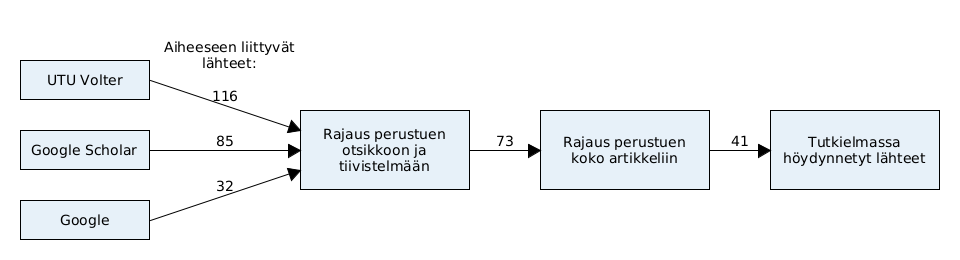
\includegraphics[width=1\textwidth]{img/lahteet.png}
\caption{Tiedonhakuprosessi\label{fig:Lahteet}}
\end{figure}

Tutkielman luvussa \ref{Raportointi ja PLM} hyödynnetään pääasiallisesti akateemisia lähteitä, jotta voidaan luoda ymmärrys PLM-strategiasta, -järjestelmistä sekä näiden yhteydestä raportointiin. Perehdymme ensin alaluvussa \ref{PLM-strategia ja PLM-järjestelmät} PLM:n merkitykseen ja sen ominaispiirteisiin. Käytämme aiempaa kirjallisuutta perustelemaan PLM:n merkityksellisyyttä ja sen yhteyttä liiketoimintatiedon hyödyntämiseen, minkä tehokas raportointi mahdollistaa.

Alaluvussa \ref{Raportointimoottorit ja -työkalut} määritellään akateemisen kirjallisuuden avulla raportointimoottorin ja -työkalun käsitteet ja rakenne. Tämän lisäksi perehdymme raportoinnin ja PLM-järjestelmän yhteyteen. Selvitämme myös, millainen PLM-järjestelmä on toimintaympäristönä ja millaisia niiden käyttäjät ovat.

Tutkielman luvussa \ref{Tapaus: Sovelia PLM:n raportointityökalu} esittelemme tapaustutkimuksen toimintaympäristön, Sovelia PLM:n, ominaisuuksia ja erityispiirteitä pohjautuen ohjelmiston dokumentaatioon. Tarkastelemme Sovelia PLM:n vanhaa raportointityökalua ja reflektoimme sen asettamia haasteita uuden raportointityökalun kehittämiselle. Tämän jälkeen perehdymme pääasiallisesti PLM-ohjelmistoja tarjoavien yritysten julkaisuihin PLM:n ja raportoinnin yhteydestä, josta päädymme tarkastelemaan kuutta olemassa olevaa raportointityökalua ja niiden ominaisuuksia. Nämä kuusi raportointityökalua valittiin, sillä niiden ominaisuudet ja toimintaympäristöt vastasivat uutta kehitettävää raportointityökalua.

Lopulta vertaamme havaintojamme kuudesta valitusta kehitettävän uuden raportointityökalun ominaisuuksiin ja erityispiirteisiin. Tämän perusteella pyrimme toteamaan, mitkä lähestymistavat soveltuivat Sovelia PLM:n tapauksessa ja mitkä eivät.

